\subsection{Color} \label{sec:color}
%
\begin{figure} [h!]
    \centering
    \begin{subfigure}[b]{0.49\textwidth}
        \centering
        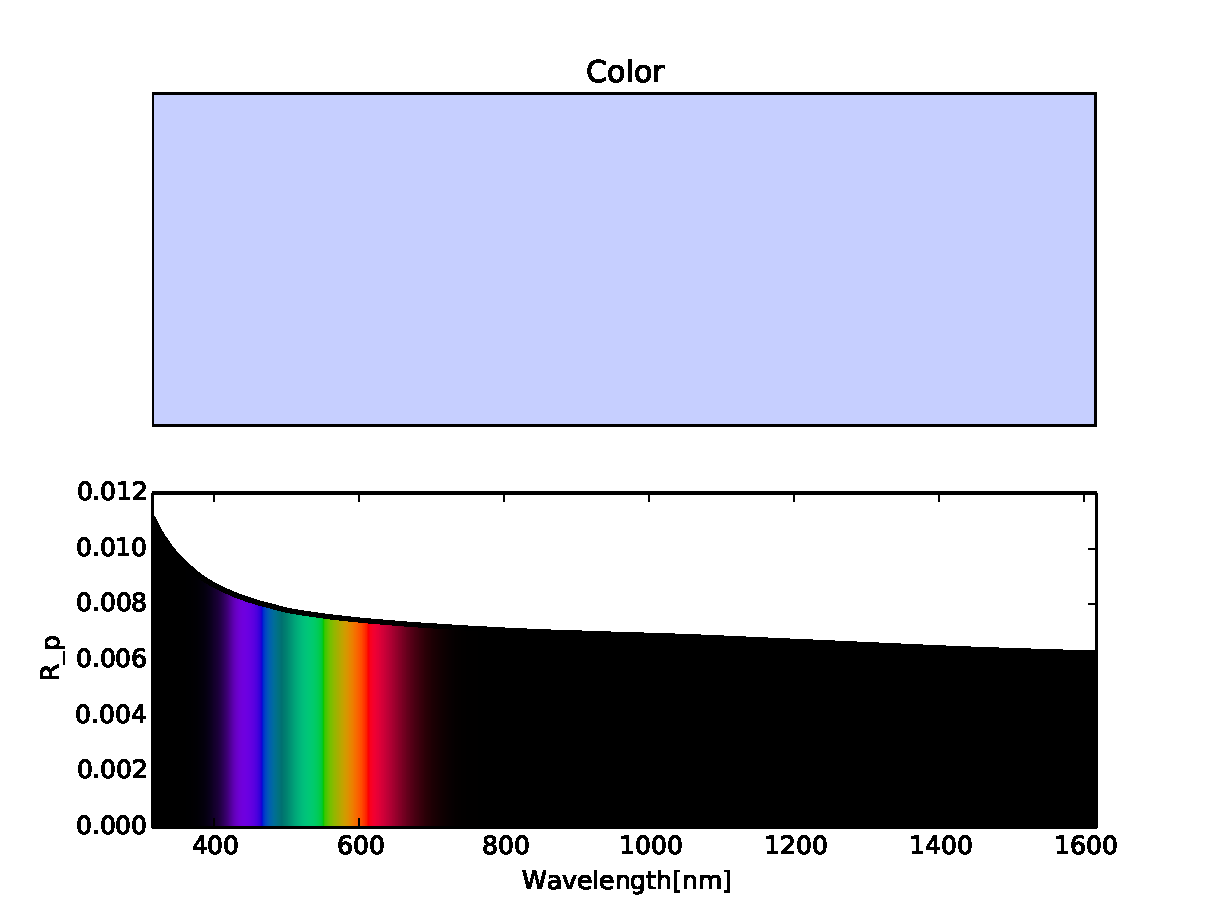
\includegraphics[width=\textwidth]{Results/Sim3/Rp_color25C.pdf}
        \caption{$T = 25^{\circ}$C}
        \label{fig:RpColor25C}
    \end{subfigure}
    %\hfill
    \begin{subfigure}[b]{0.49\textwidth}
        \centering
        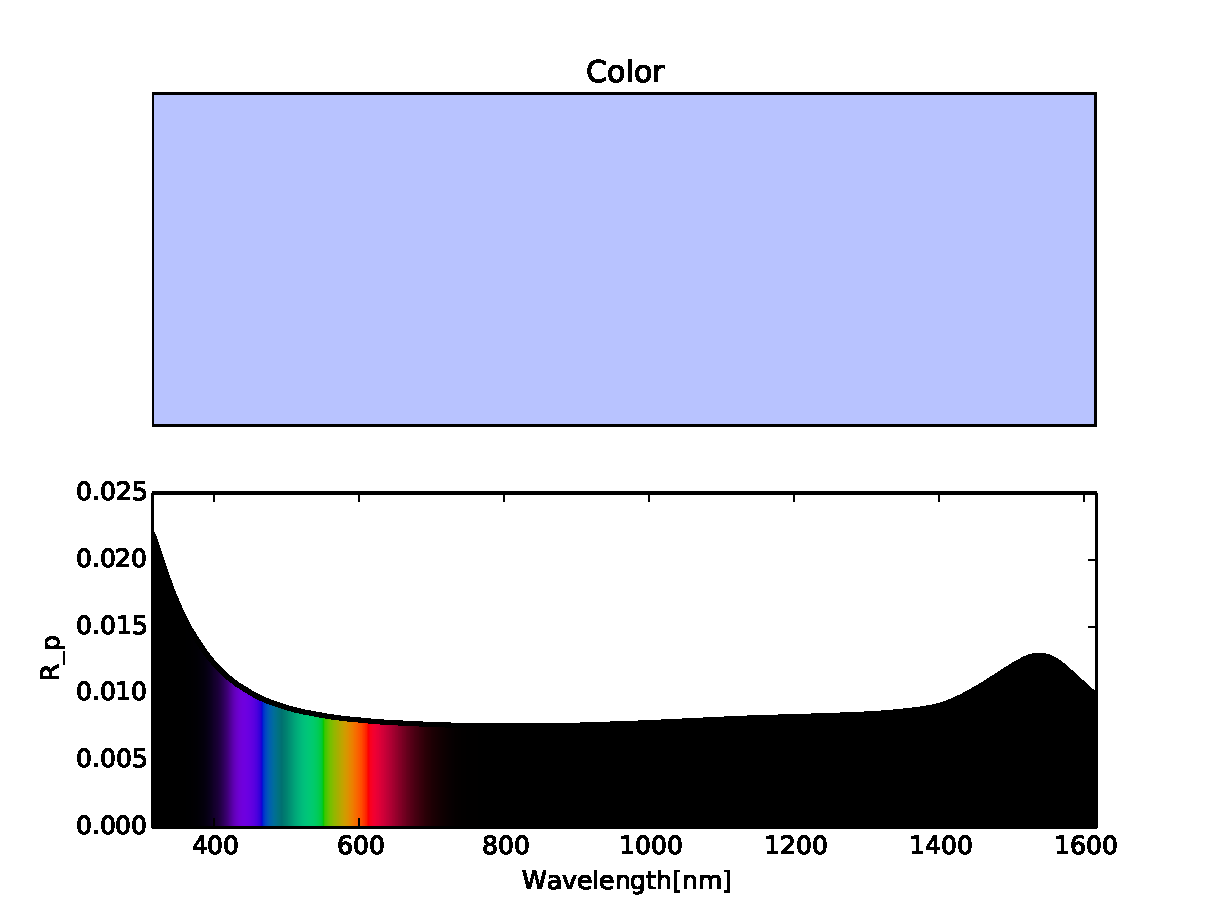
\includegraphics[width=\textwidth]{Results/Sim3/Rp_color80C.pdf}
        \caption{$T = 80^{\circ}$C}
        \label{fig:RpColor80C}
    \end{subfigure}
    \caption{
       The spectral reflectance for p-polarization together with the approximate resulting color.
       The simulation was done $r = 15$.
    }
    \label{fig:RpColor}
\end{figure}
%
%
\begin{figure}[h!]
    \centering
    \begin{subfigure}[b]{0.49\textwidth}
        \centering
        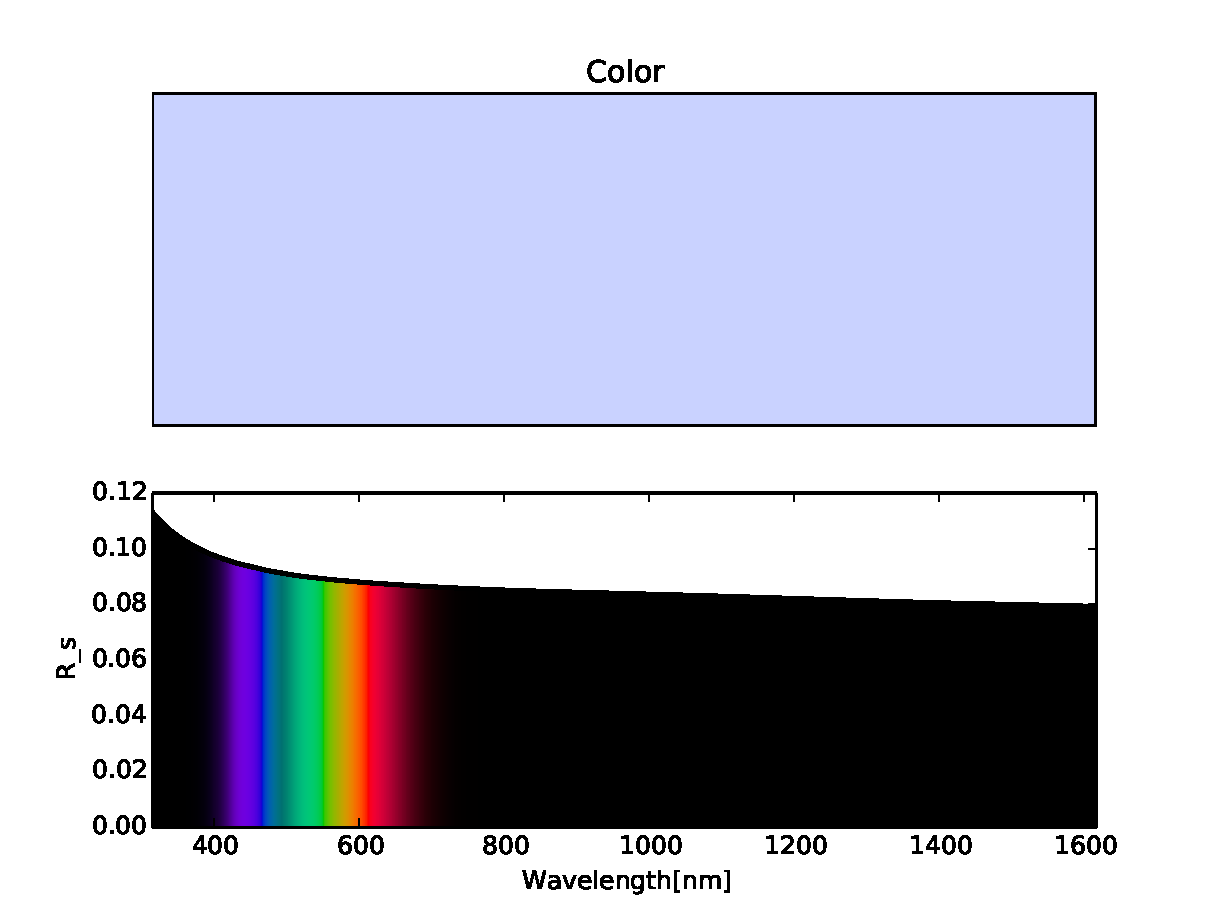
\includegraphics[width=\textwidth]{Results/Sim3/Rs_color25C.pdf}
        \caption{$T = 25^{\circ}$C}
        \label{fig:RsColor25C}
    \end{subfigure}
    %\hfill
    \begin{subfigure}[b]{0.49\textwidth}
        \centering
        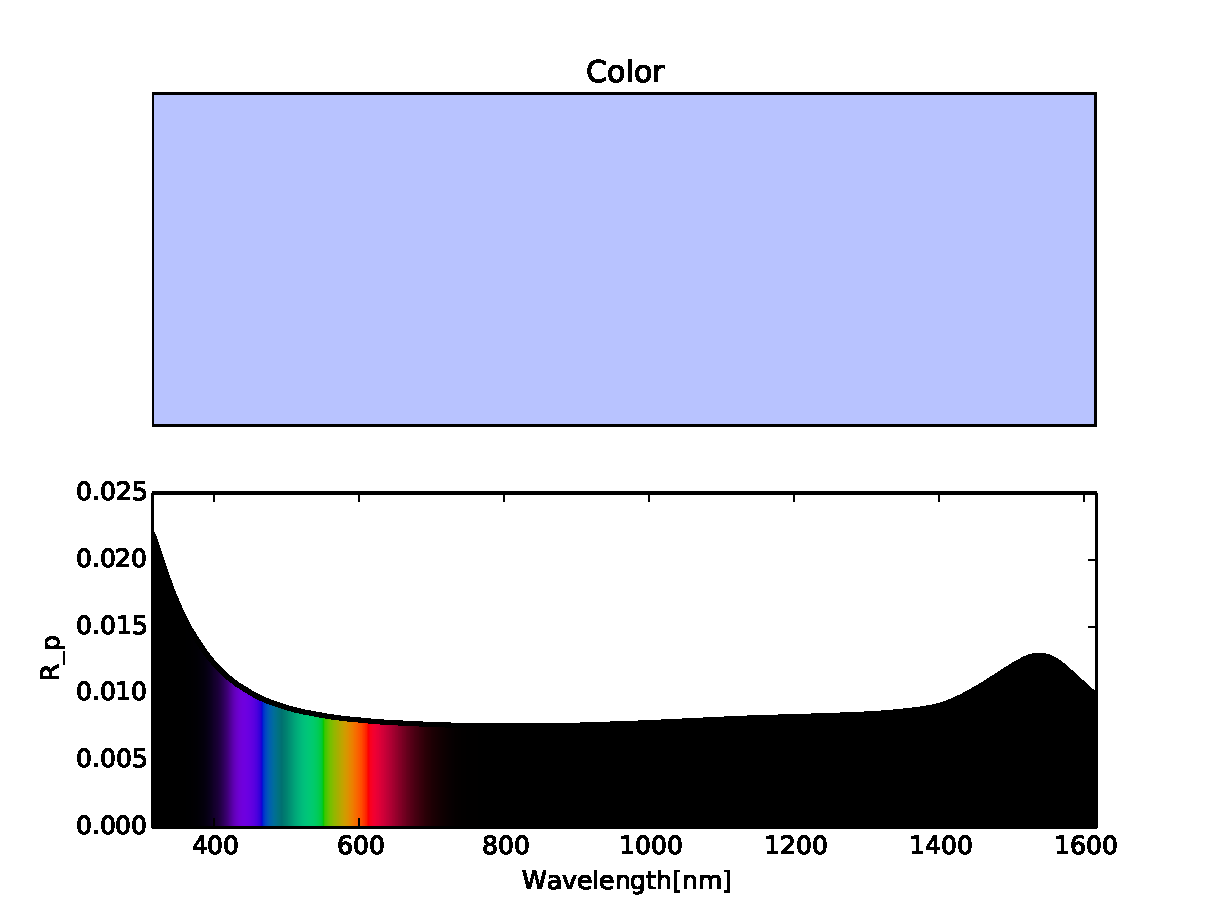
\includegraphics[width=\textwidth]{Results/Sim3/Rp_color80C.pdf}
        \caption{$T = 80^{\circ}$C}
        \label{fig:RsColor80C}
    \end{subfigure}
    \caption{
       The spectral reflectance for s-polarization together with the approximate resulting color.
       The simulation was done $r = 15$.
    }
    \label{fig:RsColor}
\end{figure}
%
%
\begin{figure}[h!]
    \centering
    \begin{subfigure}[b]{0.49\textwidth}
        \centering
        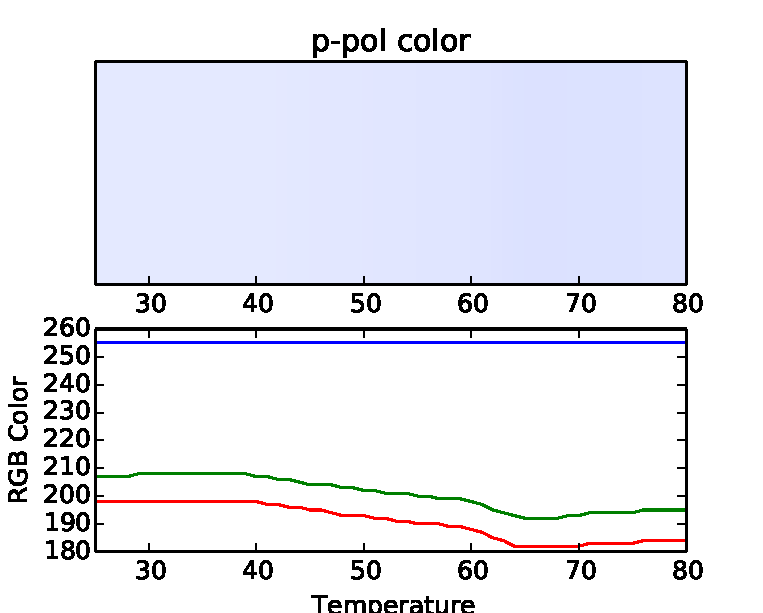
\includegraphics[width=\textwidth]{Results/Sim3/Rp_color.pdf}
        \caption{p-polarization}
        \label{fig:RpColor}
    \end{subfigure}
    %\hfill
    \begin{subfigure}[b]{0.49\textwidth}
        \centering
        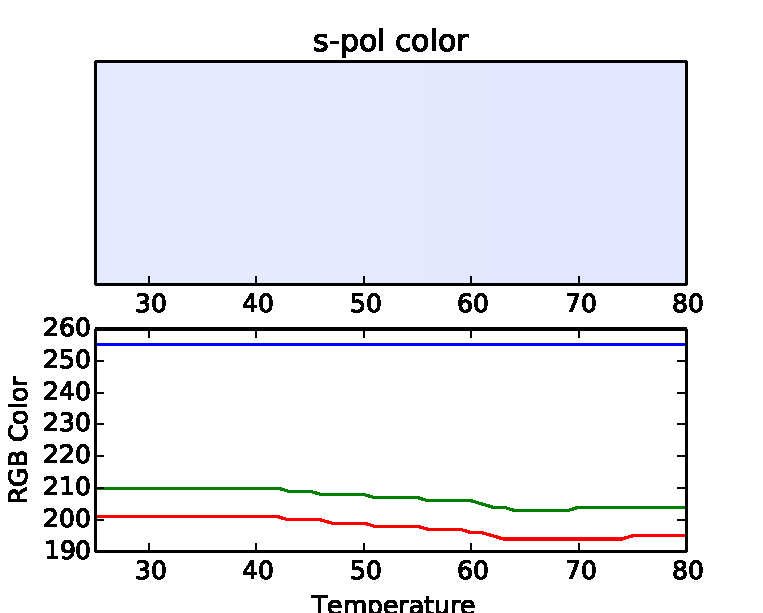
\includegraphics[width=\textwidth]{Results/Sim3/Rs_color.pdf}
        \caption{s-polarization}
        \label{fig:RsColor}
    \end{subfigure}
    \caption{
       The resulting approximated color together with the corresponding RGB values,
       based on the reflectance with $r = 15$ as a function of temperature.
    }
    \label{fig:RColor}
\end{figure}
%
